\chapter{KAJIAN PUSTAKA}


\section*{ }
Demi mendukung penelitian ini, dibutuhkan beberapa teori penunjang sebagai bahan acuan dan referensi. Dengan demikian penelitian ini menjadi lebih terarah. 
\vspace{1ex}

\section{Gumpalan Darah Vena}

Gumpalan darah atau yang biasa disebut dengan \textit{thrombus} merupakan massa padat yang terbentuk dari pembekuan darah di dalam pembuluh darah\cite{ashorobi2022thrombosis}. Adanya gumpalan darah ini yang dapat memicu terkena penyakit \textit{ Deep Vein Thrombosis} (DVT). DVT merupakan sebuah kondisi dimana adanya pembekuan darah pada daerah vena bagian dalam. Sebagian besar kasus, DVT terbentuk pada pembuluh darah pada area paha atau betis, tetapi tidak menutup kemungkinan terbentuk pada pembuluh darah pada area yang lain. 

Penyebab DVT mencakup tiga faktor utama yaitu (1) stasis vena (\textit{venous stasis}); (2) gangguan vaskular (\textit{vascular injury}); serta (3) hiperkoagulabilitas (\textit{hypercoagulability})\cite{Jonathan2017}. Stasis vena terjadi ketika aliran darah terhambat, seringkali karena kurangnya aktivitas fisik, seperti pasien yang terbaring lama atau dalam perjalanan jauh. Gangguan vaskular dapat disebabkan oleh operasi, trauma, atau inflamasi pada dinding vena. Hiperkoagulabilitas merupakan kondisi dimana darah lebih mudah untuk membeku yang disebabkan oleh beberapa faktor seperti kondisi genetik, kehamilan, atau kanker.   

Penyakit DVT harus segera didiagnosa dan ditangani secara cepat. Seringkali gejala DVT munculnya tidak secara spesifik dan bisa tidak terdeteksi. Namun, gejala umum yang muncul dari penyakit DVT dapat berupa (1) nyeri; (2) bengkak - bengkak; (3) pembuluh darah membesar di area yang terkena komplikasi jangka panjang DVT yang disebut juga dengan sindrom pascatrombotik yang dapat menyebabkan nyeri, bengkak, sensasi berat, dan kasus yang lebih parah yaitu tumbuh bisul. Berikut ini ilustrasi dari pasien yang terkena DVT yang dapat dilihat pada Gambar\ref{fig:dvtIlustration}.

\begin{figure}[H]
	\centering
	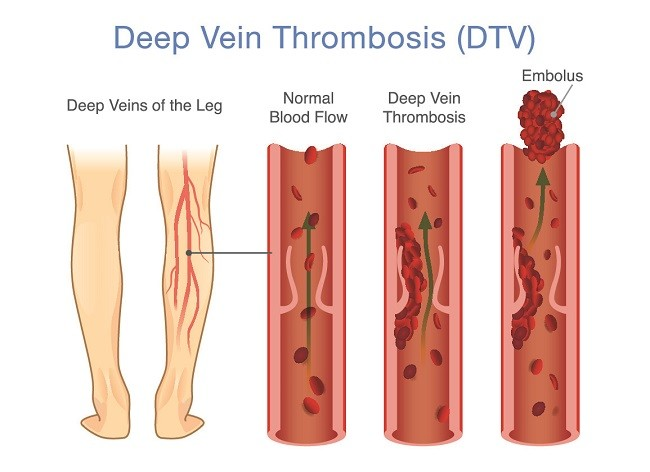
\includegraphics[scale= 0.3]{bab2/deep-vein-thrombosis.jpg}
	\caption{Ilustrasi DVT}
	\label{fig:dvtIlustration}
\end{figure}

%\underline{Menulis Dartar Item}
%\begin{itemize}
%	\item Ini Urutan Pertama. Ini Urutan Pertama. Ini Urutan Pertama. Ini Urutan Pertama. Ini Urutan Pertama. Ini Urutan Pertama. Ini Urutan Pertama. 
%	\item Menulis Item kedua.Menulis Item kedua.Menulis Item kedua.Menulis Item kedua.Menulis Item kedua.Menulis Item kedua.Menulis Item kedua.
%	\item Ini Urutan Ketiga
%\end{itemize}
%
%\underline{Menulis daftar urutan}
%\begin{enumerate}
%	\item Ini Urutan Pertama
%	\item Ini Urutan kedua
%	\begin{enumerate}
%		\item Sub Urutan Pertama
%		\item Sub Urutan Kedua
%	\end{enumerate} 
%	\item Ini Urutan Ketiga
%\end{enumerate}
\section{Citra Ultrasonografi}
Citra \textit{ultrasound} adalah citra medis yang dibuat menggunakan gelombang suara tinggi (\textit{ultrasound}) untuk memvisualisasikan organ tubuh dan struktur di dalamnya\cite{MIT2022}. Citra ini digunakan dalam bidang medis untuk tujuan diagnosis dan pemantauan kondisi kesehatan. Gambar yang dihasilkan oleh citra \textit{ultrasound} (USG) terdiri dari piksel yang mewakili gema (\textit{echo}) yang diterima oleh transduser (\textit{probe}) dan menunjukkan masing-masing bagian organ tubuh\cite{cloutier2021quantitative}. Dengan cara ini, mode ini biasanya menampilkan bagian-bagian tubuh secara rinci. \textit{Probe} yang ditempelkan pada kulit pasien mengirimkan sinyal \textit{ultrasound} ke tubuh pasien, yang kemudian merefleksikan dan menyebar, menghasilkan gema yang digunakan untuk membentuk citra \textit{ultrasound}. 

Pemrosesan citra 2D menggunakan komputer biasa disebut dengan pengolahan citra digital. Citra digital dapat dinyatakan sebagai suatu fungsi dua dimensi f(x,y), dengan x maupun y merupakan posisi koordinat sedangkan f merupakan amplitudo pada posisi(x,y) yang sering dikenal sebagai \textit{grey scale}\cite{Purnomo2010}. Citra digital dapat dibayangkan sebagai suatu matriks yang mana baris dan kolomnya merepresentasikan suatu titik di dalam citra dan nilai elemen matriks tersebut menunjukkan nilai warna pada titik tersebut. Salah satu contoh terdapat citra berukuran 128x128 piksel dengan intensitas beragam pada tiap pikselnya. Setiap pikselnya direpresentasikan secara numerik dengan matriks terdiri dari 128 baris dan 128 kolom. Nilai intensitas atau piksel bentuknya adalah diskrit mulai dari 0 hingga 255, yang mana angka 0 merupakan nilai intensitas paling gelap sedangkan angka 255 merupakan nilai intensitas yang paling terang. 

Adapun pengidentifikasian DVT oleh dokter, pencintraannya menggunakan \textit{ultrasound} jenis \textit{Doppler}. \textit{Ultrasound Doppler} merupakan proses pencitraan menggunakan gelombang suara untuk menunjukkan darah bergerak melalui pembuluh darah\cite{shah2022sonography}. \textit{Ultrasound Doppler} bekerja dengan mengukur gelombang suara yang dipantulkan dari objek bergerak seperti sel darah merah yang biasa disebut dengan efek \textit{Doppler}. Berikut ini hasil pencitraan menggunakan \textit{ultrasound Doppler} yang dapat dilihat pada Gambar \ref{fig:dopler}


\begin{figure}[H]
	\centering
	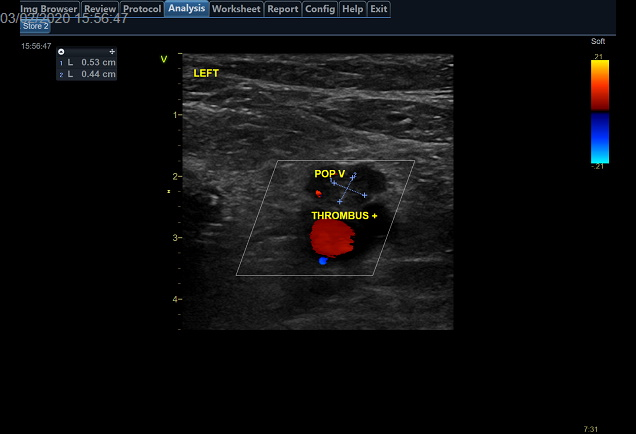
\includegraphics[scale= 0.5]{bab2/yud8Dopler.jpg}
	\caption{Hasil Pencitraan Ultrasound Dopler}
	\label{fig:dopler}
\end{figure}


%\section{Citra Ultrasonografi Tiga Dimensi}
\section{Kalibrasi}
Dalam prosedur kalibrasi menggunakan \textit{probe} \textit{ultrasound}, kami menggunakan sebuah alat yang disebut dengan kotak kalibrasi \textit{double-N}. Proses ini melibatkan beberapa langkah penting untuk memastikan keakuratan alat. Adapun prosedur pertama yaitu merancang kotak kalibrasi \textit{double-N}. Rancangan kotak kalibrasi \textit{double-N} harus sesuai dengan standar yang diperlukan agar bisa memberikan hasil kalibrasi yang tepat. Prosedur kedua yaitu melakukan desain marker pada \textit{probe} \textit{ultrasound}. Marker ini berperan penting dalam proses kalirasi karena membantu dalam menentukan koordinat objek.

Prosedur ketiga yaitu matriks kalibrasi. Prosedur ini merupakan bagian teknis yang penting dimana matriks kalibrasi ini membantu dalam mengonversi koordinat probe dan orientasi kamera \textit{optic track} menjadi informasi yang akurat. Kemudian prosedur terakhir yaitu, melakukan kalibrasi citra \textit{ultrasound}. Prosedur ini memastikan bahwa citra yang dihasilkan akurat, sehingga dapat digunakan oleh tenaga medis untuk diagnosis. Dengan demikian, setiap tahap dalam proses kalibrasi ini sangat penting untuk memastikan bahwa alat \textit{ulrasound} bekerja dengan cara yang efektif dan akurat.

\subsection{Desain Kotak Kalibrasi}
Kotak kalibrasi \textit{double-N} memiliki desain unik yang terbagi menjadi 2 bagian utama, yaitu bagian depan dan belakang. Kedua bagian tersebut tersambung melalui dua sisi yang membentuk struktur keseluruhan. Bentuknya mirip seperti balok dengan rongga di dalam dan bagian atas terbuka. Hal ini dilakukan agar kotak kalibasi tersebut dapat ditempatkan dengan mudah dalam sebuah tangki air. Untuk ukuran dari kotak kalibrasi sendiri yaitu memiliki panjang 10cm, lebar 6cm, serta tinggi 12cm dengan ketebalan dinding sebesar 0,5cm. Desain ini dirancang dengan pertimbangan khusus agar dapat berfungsi dengan baik dalam penggunaannya. Adapun desain kotak kalibrasi \textit{double-N} dapat dilihat pada Gambar \ref{fig:desain_kotak_kalibrasi} .

\begin{figure}[htbp]
	\centering
	\begin{tabular}{ll}
		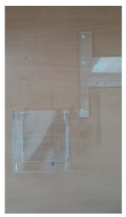
\includegraphics[scale=0.8]{bab2/kotak_sisi_belakang_kalibrasi.png}
		&
		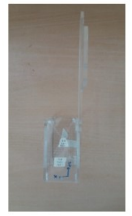
\includegraphics[scale=0.8]{bab2/kotak_sisi_samping_kalibrasi.png} \\
		\multicolumn{1}{c}{(a)} & \multicolumn{1}{c}{(b)} 
		
	\end{tabular}
	
	\begin{tabular}{ll}
		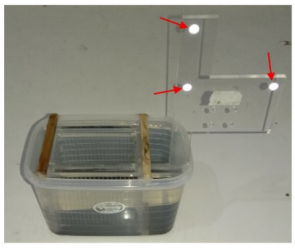
\includegraphics[scale=0.5]{bab2/kotak_kalibrasi_keseluruhan.png}\\
		\multicolumn{1}{c}{(c)}  
		
	\end{tabular}
	\caption{(a) Kotak sisi bagian belakang (b) Kotak sisi bagian samping, dan (c) Kotak kalibrasi yang diisi air}
	\label{fig:desain_kotak_kalibrasi}
\end{figure}


Kotak kalibrasi memiliki 19 lubang di sisi panjangnya, 11 di sisi lebar, serta 16 lubang pada sisi tinggi. Bagian kotak kalibrasi \textit{double-N} dilengkapi dengan benang nilon berukuran 0,45mm. Kotak bagian eksternal memiliki panjang sebesar 0,45mm, lebar 0,6mm, dan tinggi sebesar 0,7mm. Fungsi utma dari otak eksternal ini adalah untuk menampung cairan yang menjadi media untuk mentransmisikan sinyal dari \textit{probe ultrasound} ke benang. Adapun desain posisi kabel pada kotak kalibrasi dapat dilihat pada Gambar \ref{fig:desain_posisi_kabel}. 

\begin{figure}[htbp]
	\centering
	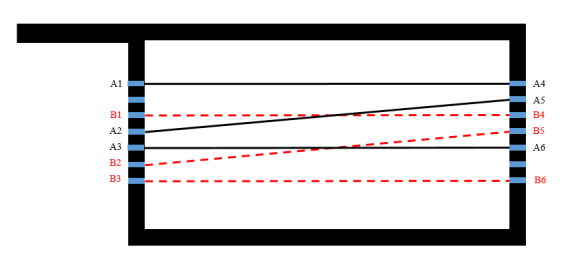
\includegraphics[scale= 0.7]{bab2/desain_posisi_kabel.png}
	\caption{Desain posisi benang pada kotak kalibrasi}
	\label{fig:desain_posisi_kabel}
\end{figure}



\subsection{Desain \textit{Marker} pada \textit{Probe}}
Marker pada \textit{probe ultrasound} memiliki 3 titik dalam sistem koordinat, yaitu M1, M2, dan M3. Titik M2 pada marker berfungsi sebagai pusat sistem koordinat pada \textit{probe ultrasound}. Sementara itu, marker pada kotak kalibrasi juga memiliki 3 titik sistem koordinat yaitu M4, M5, serta M6. Titik M6 pada marker kotak kalibrasi berfungsi sebagai pusat sistem koordinat pada kotak kalibrasi. Posisi marker dan sistem koordinat pada \textit{probe} dapat dilihat pada Gambar \ref{fig:posisi_kalibrasi}.

\begin{figure}[htbp]
	\centering
	\begin{tabular}{ll}
		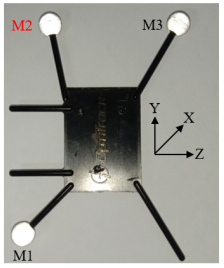
\includegraphics[scale=0.9]{bab2/marker_m2}
		&
		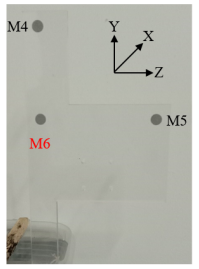
\includegraphics[scale=0.9]{bab2/marker_m6} \\
		\multicolumn{1}{c}{(a)} & \multicolumn{1}{c}{(b)}
	\end{tabular}
	\caption{(a) Posisi marker dan sistem koordinat Probe USG, M2 sebagai pusat koordinat probe. (b) Posisi marker dan sistem koordinat kotak kalibrasi, M6 sebagai pusat koordinat kotak kalibrasi.}
	\label{fig:posisi_kalibrasi}
\end{figure}




Adapun nilai dari M1, M2, dan M3 memiliki nilai yang dapat berubah - ubah. Dikarenaka adanya gerakan \textit{freehand} menggunakan \textit{probe ultrasound} saat proses kalibrasi. Namun marker M4, M5, dan M6 yang terletak pada kotak kalibrasi bersifat statis dikarenakan tidak mengikuti pergerakan \textit{freehand} \textit{probe} \textit{ultrasound}. Hasil pembacaan posisi marker, menghasilkan kumpulan titik dalam ruang tiga dimensi yang direpresentasikan dalam persamaan $M_i = x_j, y_j, z_j$. 


\subsection{Matriks Kalibrasi}
Proses ekstraksi matriks transformasi terdiri dari beberapa prosedur yang harus dilakukan. Pertama, menentukan vektor arah pada marker kotak kalibrasi. Kedua, menentukan vektor arah pada marker \textit{probe} \textit{ultrasound}. Prosedur yang terakhir yaitu menentukan matriks transformasi terhadap titik pusat marker kotak kalibrasi terhadap kamera \textit{optic track}. Titik pusat marker kotak kalibrasi direpresentasikan dengan variabel M2.

Arah vektor satuan pada sistem koordinat kotak kalibrasi didasarkan 3 sumbu yaitu $x,y,z$. Arah vektor satuan sumbu $x$ direpresentasikan dengan simbol \textbf{KX}, arah sumbu $y$ direpresentasikan dengan simbol \textbf{KY}, serta arah sumbu $z$ direpresentasikan dengan simbol \textbf{KZ}. Hal itu dapat dilihat pada Persamaan \ref{eq:persamaan_kz_1}.

\begin{equation}
	\textbf{KZ}\ =\ \frac{M5\ -\ M6}{\left|M5\ -\ M6\right|} \\
	=\ \frac{(x_5-x_6,y_5-y_6,z_5-z_6)}{\sqrt{{(x_5-x_6)}^2\ +\ {(y_5-y_6)}^2\ +\ {(z_5-z_6)}^2\ \ }}
	\label{eq:persamaan_kz_1}
\end{equation}

Dalam mengukur vektor satuan ke arah sumbu $x$ atau $KX$ dalam sistem koordinat kotak kalibrasi dibutuhkan Persamaan \ref{eq:persamaan_kx_1}. Kemudian variabel $KS$ merupakan vektor yang menggambarkan perpindahan dari titik $M4$ ke titik $M6$.

\begin{equation}
	\begin{aligned}
		\textbf{KX}\ =\ KS\ \times\ KZ \\[20pt]
		\textbf{KS}\ =\ M4\ -M6 =\ (x_4-x_6,y_4-y_6,z_4-z_6) \\[20pt] 
		\texbf{KX}\ =\ \frac{x_{KX}{,y}_{KX}{,z}_{KX}}{\sqrt{{(x_{KX})}^2+{(y_{KX})}^2+{(z_{KX})}^2}}
	\end{aligned}
	\label{eq:persamaan_kx_1}
\end{equation}

Adapun dalam mengukur vektor satuan ke arah sumbu $y$ ($KY$) dalam sistem koordinat kotak kalibrasi dibutuhkan Persamaan \ref{eq:persamaan_ky_1}. 

\begin{equation}
	\begin{aligned}
		\textbf{KY} = KZ \times KX \\[20pt]
		 \texbf{KY}\ =\ \frac{x_{KY}{,y}_{KY}{,z}_{KY}}{\sqrt{{(x_{KY})}^2+{(y_{KY})}^2+{(z_{KY})}^2}}
	\end{aligned}
	\label{eq:persamaan_ky_1}
\end{equation}  

Kemudian, hasil matrik transformasi yang diperoleh dengan titik pusat M6 terhadap sistem koordinat kamera \textit{optic track} (${_T^H}T$) dapat dilihat pada Persamaan \ref{eq:persamaan_matriks_m6}.

\begin{equation}
	{_T^H}T = \begin{bmatrix}x_{KX} & y_{KX} & z_{KX} & M6_x  \\x_{KY} & y_{KY} & z_{KZ} & M6_y \\x_{KZ} & y_{KZ} & z_{KZ} & M6_z \\0 & 0 & 0 & 1 \end{bmatrix}	
	\label{eq:persamaan_matriks_m6}
\end{equation}

Sementara itu, arah vektor satuan pada sistem koordinat \textit{probe ultrasound} didasarkan pada 3 sumbu yaitu $X$, $Y$, dan $Z$. Dalam mengukur vektor satuan ke arah sumbu $Z$ (\textbf{PZ}) dihitung berdasarkan Persamaan \ref{eq:persamaan_z_probe}.

\begin{equation}
	\textbf{PZ} = \frac{M3 - M2}{\left|M3 - M2 \right|} = \frac{(x_3-x_2, y_3 - y_2, z_3 - z_2)}{\sqrt{{(x_3 - x_2)^2 + (y_3 - y_2)^2 + (z_3 - z_2)^2 }}}
	\label{eq:persamaan_z_probe}
\end{equation} 

Dalam mengukur vektor satuan ke arah sumbu $X$ (\textbf{PX}) dihitung berdasarkan Persamaan \ref{eq:persamaan_px_probe}. Dimana \textbf{PS} merupakan vektor dari M1 terhadap M2 yang ditunjukkan pada Persamaan \ref{eq:persamaan_ps_probe}.

\begin{equation}
	\textbf{PS} = M1 - M2 = (x_1 - x_2, y_1 - y_2, z_1 - z_2)
	\label{eq:persamaan_ps_probe}
\end{equation}

\begin{equation}
	\begin{align}
		\textbf{PX} = \textbf{PS} \times \textbf{PZ}\\[10pt]
		\textbf{PX} = \frac{(x_{PX}, y_{PX}, z_{PX})}{\sqrt{{(x_{PX})^2 + (y_{PX})^2 + (z_{PX})^2}}}
	\end{align}
	\label{eq:persamaan_px_probe}
\end{equation}

Sementara itu, untuk mengukur vektor satuan ke arah sumbu $Y$ (\textbf{PY}) pada sistem koordinat \textit{probe ultrasound} dihitung berdasarkan Persamaan \ref{eq:persamaan_py_probe}. Dimana nilai vektor satuan \textbf{PY} diperoleh dari hasil perkalian antara vektor satuan ke arah sumbu $Z$ (\textbf{PZ}) dengan vektor satuan ke arah sumbu $X$ (\textbf{PX}).

\begin{equation}
	\begin{align}
		\textbf{PY} = \textbf{PZ} \times \textbf{PX} \\
		\textbf{PY} = \frac{(x_{PY}, y_{PY}, z_{PY})}{\sqrt{{(x_{PY}^2 + (y_{PY}^2 + (z_{PY}^2)}}}
	\end{align}	
	\label{eq:persamaan_py_probe}
\end{equation}

Dari perhitungan vektor satuan dari masing - masing arah sumbu $X$,$Y$,$Z$ pada sistem koordinat \textit{probe ultrasound}. Diperoleh matrik transformasi dari titik pusat M2 terhadap sistem koordinat \textit{probe ultrasound} (${_T^P}T$) dapat dilihat pada Persamaan \ref{eq:persamaan_matriks_m2}.


\begin{equation}
	{_T^P}T = \begin{bmatrix}x_{PX} & y_{PX} & z_{PX} & M2_x  \\x_{PY} & y_{PY} & z_{PZ} & M2_y \\x_{PZ} & y_{PZ} & z_{PZ} & M2_z \\0 & 0 & 0 & 1 \end{bmatrix}	
	\label{eq:persamaan_matriks_m2}
\end{equation}

Selanjutnya, citra \textit{ultrasound} (\textbf{U}) diubah melalui proses transformasi terhadap \textit{probe ultrasound} (\textbf{P}) menggunakan teknik transformasi homogen. Proses transformasi tersebut direpresentasikan dalam simbol $T{_U^P}$. Dengan menggunakan transformasi homogen, dapat diperoleh perubahan yang diperlukan pada citra \textit{ultrasound} untuk disesuaikan dengan posisi \textit{probe ultrasound}.



\subsection{Kalibrasi Skala Citra \textit{Ultrasound}}
Proses kalibrasi pada citra \textit{ultrasound} merupakan langkah penting untuk memastikan bahwa ukuran yang ditampilkan dalam citra tersebut sesuai dengan ukuran sebenarnya. Dalam hal ini, proses kalibrasi berfungsi untuk menentukan seberapa panjang setiap piksel dalam citra \textit{ultrasound} yang dihubungkan dengan ukuran nyata dalam satuan metrik.

Untuk melakukan kalibrasi ini diperlukan penggunaan perangkat lunak seperti \textit{Echo Wave II}. Perangkat lunak ini memungkinkan untuk mengambil pengukuran yang diperlukan dari citra yang dihasilkan. Kalibrasi ini dilakukan dengan mengukur skala citra baik secara horizontal maupun vertikal. Pengukuran secara horizontal ditandai dengan $S_x$ sedangkan pengukuran secara vertikal ditandai dengan $S_y$. Adapun pengukuran skala citra secara horizontal dan vertikal dapat dilihat pada Persamaan \ref{eq:persamaan_skala_citra}.

\begin{equation}
	\begin{aligned}
		S_x &= \frac{D_{px}}{D_{mx}} \\[10pt]
		S_y &= \frac{D_{py}}{D_{my}}
	\end{aligned}
	\label{eq:persamaan_skala_citra}
\end{equation}

Dimana variabel $D_{px}$ menunjukkan panjang piksel secara horizontal, $D_{mx}$ menunjukkan panjang metrik secara horizontal, $D_{py}$ menunjukkan panjang piksel secara vertikal, serta $D_{my}$ menunjukkan panjang metrik secara vertikal. Dalam proses pengukuran yang dilakukan menggunakan perangkat lunak \textit{Echo Wave II}, ditetapkan pengaturan kedalaman (\textit{depth}) sebesar 40. Ini memungkinkan untuk mendapatkan pengukuran yang akurat dalam satuan milimeter. Pengukuran ini dilakukan sejauh 20mm mengikuti garis lurus baik secara horizontal maupun vertikal. Setelah mendapatkan hasil pengukuran, langkah berikutnya yaitu membandingkannya dengan ukuran piksel pada citra yang dihasilkan oleh perangkat lunak. Hal ini dilakukan dengan mengukur jarak pikel dari ujung awal hingga ujung akhir secara horizontal dan vertikal. Adapun citra hasil pengukuran pada perangkat lunak \textit{Echo Wave II} dapat dilihat pada Gambar \ref{fig:result_echo_wave}.


\begin{figure}[htbp]
	\centering
	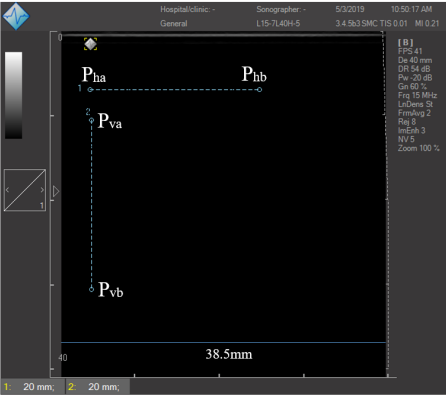
\includegraphics[scale= 0.6]{bab2/hasil_echo_wave.png}
	\caption{Citra hasil pengukuran menggunakan perangkat lunak \textit{Echo Wave II}}
	\label{fig:result_echo_wave}
\end{figure}

Dari hasil pengukuran yang telah dilakukan, ditemukan beberapa titik koordinat posisi. Posisi $P_ha(u_{xha}, v_{xha})$ = (133, 130), $P_hb(u_{xhb}, v_{xhb})$ = (383, 130), $P_va(u_{xva}, v_{xva})$ = (135,175) serta $P_vb = (135, 425)$. Dengan menggunakan data koordinat tersebut dan menerapkan persamaan \ref{eq:persamaan_jarak_koordinat} dapat menghitung panjang piksel. Adapun perhitungan panjang piksel menggunakan persamaan \ref{eq:persamaan_jarak_koordinat} diperoleh hasil panjang piksel secara horizontal $D_{px} =$ 250 piksel dan panjang piksel secara vertikal $D_{py} =$ 250 piksel.   


\begin{equation}
	\begin{aligned}
		D_{px} = \sqrt{(u_{xhb} - u_{xha})^2 + (v_{xhb} - v_{xha})^2 } \\[10pt]
		D_{py} = \sqrt{(u_{yhb} - u_{yha})^2 + (v_{yhb} - v_{yha})^2 }
	\end{aligned}
	\label{eq:persamaan_jarak_koordinat}
\end{equation} 

Dalam pengukuran ini diperoleh nilai panjang metrik secara horizontal $D_{mx}$ sebesar 20mm dan panjang metrik secara vertikal $D_{my}$ sebesar 20mm. Dari hasil tersebut, perbandingan skala secara horizontal $S_x$ = 20mm/250 piksel, sehingga didapatkan 1 piksel = 0,08mm. Perbandingan skala vertikal $S_y$ = 20mm/250 piksel sehingga 1 piksel =0,08mm.

%
%\section{Rekonstruksi 3D Citra \textit{Ultrasound}}
\section{Peningkatan Kualitas Citra}
Salah satu kelemahan dari citra \textit{ultrasound} sendiri adalah memiliki banyak \textit{noise}. Efek \textit{noise} yang berulang (\textit{multiplicative}) yang dilihat dalam bentuk granular (bintik) biasa disebut dengan \textit{speckle}\cite{made2020}. Tubuh menghasilkan \textit{speckle} dari kejadian terus-menerus dan sinyal pantul. Struktur dan karakteristik \textit{speckle} biasanya bergantung pada jaringan yang dicitrakan. Pengurangan \textit{speckle} sangat penting untuk meningkatkan kualitas dan pemahaman kita tentang pencitraan medis menggunakan \textit{ultrasound}. Adapun beberapa penelitian relevan terkait penghapusan \textit{noise} pada citra \textit{ultrasound}.

Penelitian yang dilakukan oleh Shodiq, dkk (2022)\cite{shodiq2022} membandingkan beberapa filter reduksi \textit{speckle} pada citra \textit{ultrasound} pembuluh darah serta memprediksi area pembuluh darah menggunakan model \textit{deep learning} U-Net. Adapun filter reduksi \textit{speckle} yang dibandingkan sebagai berikut (1) \textit{Wiener Filtering}; (2) \textit{Lee Filtering}; (3) \textit{Non-local means Filtering}; (4) \textit{Median Filtering}; (5) \textit{Total Variation Filter}; (6) \textit{Anisotropic Diffusion Filtering}; (7) \textit{Gaussian Filter}; serta (8) \textit{Wafelet Filter}. Adapun hasil penelitian yang diperoleh yaitu citra 2D \textit{ultrasound} gumpalan darah yang melalui proses reduksi \textit{speckle} dengan menggunakan filter \textit{Gaussian} mendapat hasil terbaik daripada beberapa filter reduksi \textit{speckle} yang lain dengan rata - rata akurasi sebesar 99\%, rata - rata nilai \textit{loss parameter} sebesar 0.0252, rata - rata nilai akurasi IoU sebesar 84.9\%,serta rata - rata nilai \textit{Hausdorff distance} sebesar 4.17. Prediksi \textit{mask area} menggunakan model \textit{deep learning} U-Net dengan filter \textit{gaussian} mendapat nilai 99.4\%.



\section{Segmentasi Citra \textit{Ultrasound}}
Segmentasi citra adalah teknik yang membagi citra digital menjadi subkelompok yang disebut segmen citra. Secara teknis, segmentasi adalah memberi label ke setiap piksel untuk menunjukkan objek, orang, atau elemen penting lainnya. Teknik ini biasanya digunakan untuk deteksi objek\cite{Yanhui2019}. Untuk menemukan objek yang diinginkan, algoritma segmentasi citra biasanya digunakan. Setelah objek ditemukan, detektor objek dapat beroperasi pada Region of Interest (RoI) yang telah ditentukan oleh algoritma tersebut. RoI itu sendiri mengurangi waktu inferensi dan meningkatkan akurasi. 

Output segmentasi citra merupakan kumpulan matriks atau mask dengan berbagai elemen yang menentukan kelas objek atau instance yang dimiliki setiap piksel\cite{kurmann2021mask}. Untuk segmentasi citra, mungkin bermanfaat untuk menggunakan beberapa heuristik yang relevan atau fitur gambar berkualitas tinggi. Algoritma segmentasi citra standar yang menggunakan teknik pengelompokan fitur tepi dan histogram bergantung pada fitur-fitur ini. Fitur warna merupakan salah satu contoh heuristik yang populer dalam proses segmentasi. Kontras program segmentasi citra juga bermanfaat karena dapat dengan mudah membedakan antara gelap dan terang.Teknik segmentasi citra tradisional yang bergantung pada heuristik semacam itu dapat dilakukan dengan cepat dan mudah, tetapi teknik tersebut sering kali memerlukan penyempurnaan untuk mendukung penggunaan heuristik yang dirancang secara manual dalam situasi tertentu\cite{jena2018survey}.

%\subsection{\textit{Machine Learning}}
%
%\subsection{\textit{Deep Learning}}
 
\subsection{Convolutional Neural Network (CNN)}
Salah satu jenis jaringan saraf tiruan yang digunakan untuk pengolahan data citra adalah Convolutional Neural Network (CNN). CNN menggunakan konsep konvolusi untuk mengekstrak karakteristik penting dari citra input, yang memungkinkan proses klasifikasi citra. CNN terdiri dari berbagai layer, termasuk layer convolution, layer pooling, dan layer fully-connected\cite{Mayank2020}. Layer pooling mengurangi overfitting sekaligus mengurangi dimensi feature map yang dibuat oleh layer convolution sebelumnya, dan layer convolution digunakan untuk mengekstrak fitur dari citra dengan menggunakan filter konvolusi yang diterapkan pada setiap sub-regional dari citra. Lapisan fully-connected mengklasifikasikan citra berdasarkan karakteristik yang diekstrak dari deretan layer sebelumnya.
CNN sudah banyak digunakan dalam bermacam aplikasi pengolahan citra semacam klasifikasi citra, deteksi objek, serta lain- lain. Beberapa penelitian relevan yang mengulas tentang CNN pada citra kedokteran antara lain sebagai berikut

Penelitian yang telah dilakukan oleh Sudha, dkk (2019)\cite{sudha2019} menunjukkan segmentasi area \textit{mask} citra arteri karotis menggunakan model CNN. Adapun hasil penelitian yang diperoleh yaitu model CNN lebih efektif digunakan untuk segmentasi daripada model SVM classifier dan model \textit{Radial Basis Function} dengan tingkat akurasi sebesar 99.33\%.


\subsection{U-Net - Deep Learning Model}
U-Net merupakan salah satu model \textit{deep learning} yang digunakan dalam segmentasi citra medis, khususnya pada citra 2D USG. Model U-Net dikembangkan oleh Olaf Ronneberger, dkk (2015) \cite{ronneberger2015u} dalam paper yang berjudul \textit{"U-Net: Convolutional Networks for Biomedical Image Segmentation"}.  Adapun keunggulan model U-Net sebagai model segmentasi sebagai berikut:
\begin{enumerate}
	\item U-Net telah terbukti memberikan hasil segmentasi yang baik dalam citra medis, dan karenanya sering digunakan dalam berbagai aplikasi segmentasi citra medis, termasuk citra ultrasound, MRI, dan CT-Scan.
	\item U-Net memiliki parameter yang lebih sedikit daripada model deep learning lainnya, sehingga pelatihannya menjadi lebih mudah dan waktu komputasinya lebih singkat.
	\item U-Net mengadaptasi arsitektur \textit{encoder} dan \textit{decoder}. Pada \textit{encoder} U-Net mengadaptasi arsitektur \textit{encoder} yang bertugas untuk mengekstraksi fitur - fitur tingkat tinggi dari citra. Sedangkan \textit{decoder} U-Net bertugas untuk mengembalikan informasi spasial ke dimensi asli citra untuk menghasilkan prediksi segmentasi.
	\item U-net juga memanfaatkan \textit{skip connection} yang menghubungkan bagian \textit{encoder} dan \textit{decoder}. Hal ini dapat membantu meningkatkan kemampuan segmentasi pada tingkat resolusi yang lebih rendah.
 \item U-Net dapat digunakan segmentasi \textit{multiclass} pada citra dua dmensi. Model ini dapat dilatih untuk mengidentifikasi dan memisahkan beberapa struktur atau objek yang berbeda dalam citra dua dimensi, seperti organ.
\end{enumerate}

% Penelitian yang dilakukan oleh Abdollahi, dkk (2020)\cite{abdollahi2020} bertujuan untuk segmentasi citra area jalan raya di Massachusets (negara bagian Amerika Serikat) dan Ottawa (Kanada). Yang menjadi tantangan dalam penelitian ini adalah citra yang akan disegmentasi memiliki resolusi yang tinggi serta segementasi area yang termasuk bagian dari jalan seperti bangunan, pohon, pejalan kaki, kendaraan, jalan pedesaan. Kelas - kelas tersebut memiliki karakteristik yang heterogen. Peneliti menggunakan model V-Net dengan menambahkan parameter \textit{Cross Entropy Dice Loss} (CEDL) yang digunakan untuk segmentasi area jalan. Hasil penelitian ini menyebutkan bahwa hasil akurasi segmentasi area jalan mendapatkan nilai 90.64\% untuk dataset Massachusetss serta 92.41\% untuk dataset Ottawa. Pada penelitian juga mengkomparisikan hasil akurasi menggunakan U-Net + CEDL dengan model FCN, Segnet, dan U-Net dimana masing - masing mendapatkan akurasi sebesar 1.09\%, 2.45\%, dan 0.39\% untuk dataset Massachusets. Kemudian nilai 7.21\%, 1.86\%, dan 2.68\% untuk dataset Ottawa.
Penelitian yang telah dilakukan oleh Yang, dkk (2022)\cite{yang2022ax}
melakukan segmentasi pankreas. Dalam penelitian ini, peneliti mengusulkan model segmentasi yaitu AX-Unet yang merupakan U-Net termodifikasi dengan memadatkan piramida untuk mempelajari informasi lokai dan mengekstrak informasi kontekstual multi-level untuk mengurangi kehilangan informasi selama pengurangan sampel. Peneliti juga memperkenalkan konvolusi baru pada peta fitur di setiap level untuk mencapai pemisahan informasi antar saluran. Kemudian peneliti juga mengusulkan fungsi batas eksplisit guna mengatasi batas buram. Data yang digunakan dalam penelitian ini adalah dataset \textit{Pancreas}-CT publik, dataset NIH-Pancreas-CT, serta datataset pankreas medis \textit{decathlon}. Hasil eksperimen menunjukkan bahwa model yang diusulkan oleh peneliti dapat mengungguli metode terbaru dalam segmentasi citra CT Pankreas. Dengan membandingkan output fitur yang diekstraksi dari model yang diusulkan, peneliti menemukan bahwa daerah pankreas pada orang normal dan pasien penderita tumor pankreas menunjukkan perbedaan yang signifikan.

Penelitian yang dilakukan oleh Behboodi, dkk (2019)\cite{behboodi2019ultrasound} mengusulkan penggunaan citra \textit{ultrasound} sebagai dataset untuk \textit{training} pada model \textit{deep learning} U-Net yang diujikan pada data yang diakuisisi melalui phantom. Kontribusi penelitian ini, peneliti melatih menggunakan data \textit{envelope} dan citra B-Mode.

% Penelitian yang dilakukan oleh Dangoury, dkk\cite{Dangoury2022} menguji implementasi model V-Net dalam segmentasi citra dua dimensi \textit{ultrasound}. Tidak hanya itu, hasil dari penelitian tersebut dibandingkan dengan model U-Net dan model U-Net++ berdasarkan empat \textit{Loss Function} seperti \textit{ Cross-Entropy (CE)}, \textit{Dice Similarity Coefficient} (DSC), Focal loss (FL) and \textit{Focal Tversky Loss}. 

Model U-Net memiliki tiga lapisan utama yaitu \textit{encoder}, \textit{skip connection}, dan \textit{decoder}. Pada bagian \textit{encoder} berfungsi untuk mengimplementasikan fitur setiap layer pada citra input. Kemudian bagian \textit{decoder} berfungsi untuk mengubah fitur yang menjadi output pada bagian \textit{encoder} menjadi citra prediksi \textit{mask}. Bagian \textit{skip connection} berfungsi untuk menghubungkan bagian \textit{encoder} dengan \textit{decoder} pada model U-Net. Adapun langkah - langkah model U-Net sebagai berikut:
\begin{enumerate}
    \item Citra dimasukkan ke dalam layer pada bagian \textit{encoder}.
    \item Citra akan diekstraksi fiturnya oleh setiap layer yang ada pada bagian \textit{encoder}.
    \item Output dari bagian \textit{encoder} berupa fitur dikirimkan ke bagian \textit{decoder} melalui \textit{skip connection}.
    \item Layer - layer yang ada pada bagian \textit{decoder} menggabungkan fitur menjadi citra prediksi \textit{mask}.
    \item Hasil prediksi \textit{mask} menjadi output dari segmentasi menggunakan model U-Net.
\end{enumerate}

\begin{figure}[htbp]
	\centering
	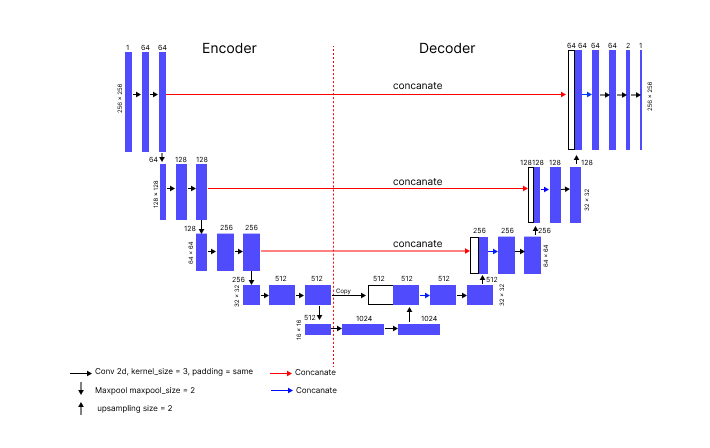
\includegraphics[scale= 0.6]{bab2/mondelUnetBab2.png}
	\caption{Arsitektur U-Net}
	\label{fig:modelU-Net}
\end{figure}

%\subsection{Konfigurasi \textit{Hyperparameter}}
%\subsubsection{\textit{Epoch}}
%\subsubsection{\textit{Batch}}
%\subsubsection{\textit{Iterasi}}
%\subsubsection{\textit{Optimizer}}
%\subsubsection{\textit{Loss Function}}
%\subsubsection{\textit{Activation Function}}



\subsection{Metric Evaluation}
\subsubsection{Akurasi}
Akurasi merupakan metrik evaluasi yang mengukur efisiensi suatu model pembelajaran mesin dalam menghasilkan prediksi yang valid. Adapun akurasi dapat dilihat pada persamaan berikut. 

\begin{equation}
	\text{Akurasi} = \frac{TP + TN}{TP + TN + FP + FN}
\end{equation}

\subsubsection{Intersection Over Union (IOU)}
\textit{Intersection over Union} (IoU) digunakan untuk mengukur kemiripan antara dua objek 2D dalam sebuah citra\cite{rezatofighi2019generalized}. Nilai IoU diperoleh melalui perhitungan area irisan antara area objek yang sebenarnya (\textit{ground-truth}) ($X$) dengan area yang dihasilkan oleh model segmentasi (\textit{masking predicted}) ($Y$). Kemudian hasil perhitungan area irisan antara dua objek tersebut dibagi dengan hasil perhitungan area gabungan dari 2 objek tersebut. Adapun persamaan IoU dapat dilihat pada Persamaan \ref{eq:persamaan1}. 

\begin{equation}
	\label{eq:persamaan1}
	\textit{IoU} = \frac{\textit{Area Irisan (Intersection)}}{\textit{Area Gabungan (Union)}} = \frac{|\ X \cap Y\ |}{|\ X \cup Y\ |}
\end{equation}


Hasil pengukuran IoU terdiri dari rentang nilai mulai dari 0 hingga 1. Apabila nilai IoU mendekati nilai 0, maka hasil prediksi segmentasi tidak mirip dengan bentuk \textit{ground truth}. Sebaliknya, apabila perhitungan IoU mendekati nilai 1, maka hasil prediksi segmentasi mirip dengan \textit{groundtruth}.

\begin{figure}[htbp]
	\centering
	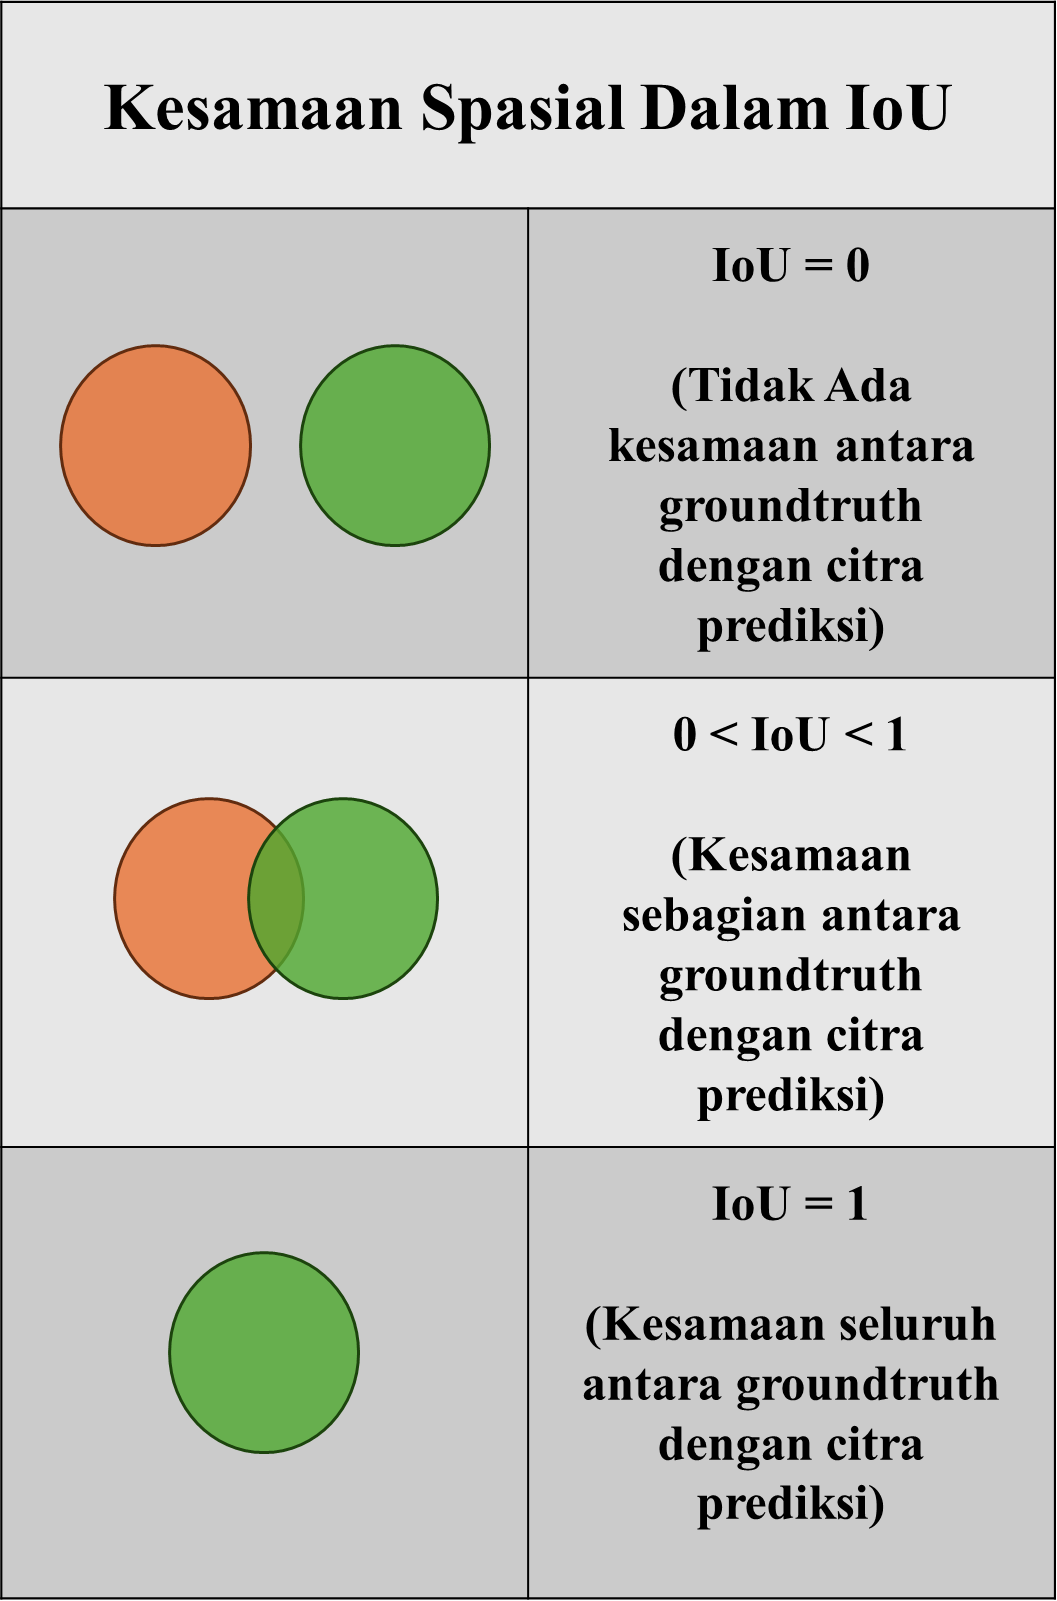
\includegraphics[scale= 0.2]{bab2/iou_spasial.png}
	\caption{Representasi Kesamaan dalam nilai IoU}
	\label{fig:iou_spasial}
\end{figure}

\subsubsection{\textit{Dice Coefficient}}
\textit{Dice coefficient} merupakan metrik evaluasi digunakan untuk mengukur tingkat kesesuaian antara 2 citra yaitu citra area objek sebenarnya(\textit{ground-truth}) dengan citra prediksi dari hasil segmentasi. Nilai \textit{dice coefficient} diperoleh dari 2 kali ukuran area irisan antara area objek yang sebenarnya (\textit{ground-truth}) ($X$) dengan area yang dihasilkan oleh model segmentasi (\textit{masking predicted}) ($Y$). Kemudian hasil perhitungan dua kali area irisan antara dua objek tersebut dibagi dengan hasil perhitungan area gabungan dari 2 objek tersebut. Adapun perhitungan \textit{dice coefficient} dapat dirumuskan sebagai berikut. 

\begin{equation}
	\textit{Dice(X,Y)} = \frac{2 \times \textit{Area Irisan (Intersection)}}{\textit{Area Gabungan (Union)}} = \frac{|\ X \cap Y\ |}{|\ X \cup Y\ |}
\end{equation}

Hasil pengukuran \textit{dice coefficient} terdiri dari rentang nilai mulai dari 0 hingga 1. Apabila nilai \textit{dice coefficient} mendekati nilai 0, maka hasil prediksi segmentasi tidak mirip dengan bentuk \textit{ground truth}. Sebaliknya, apabila perhitungan \textit{dice score} mendekati nilai 1, maka hasil prediksi segmentasi mirip dengan \textit{groundtruth}.

\begin{figure}[htbp]
	\centering
	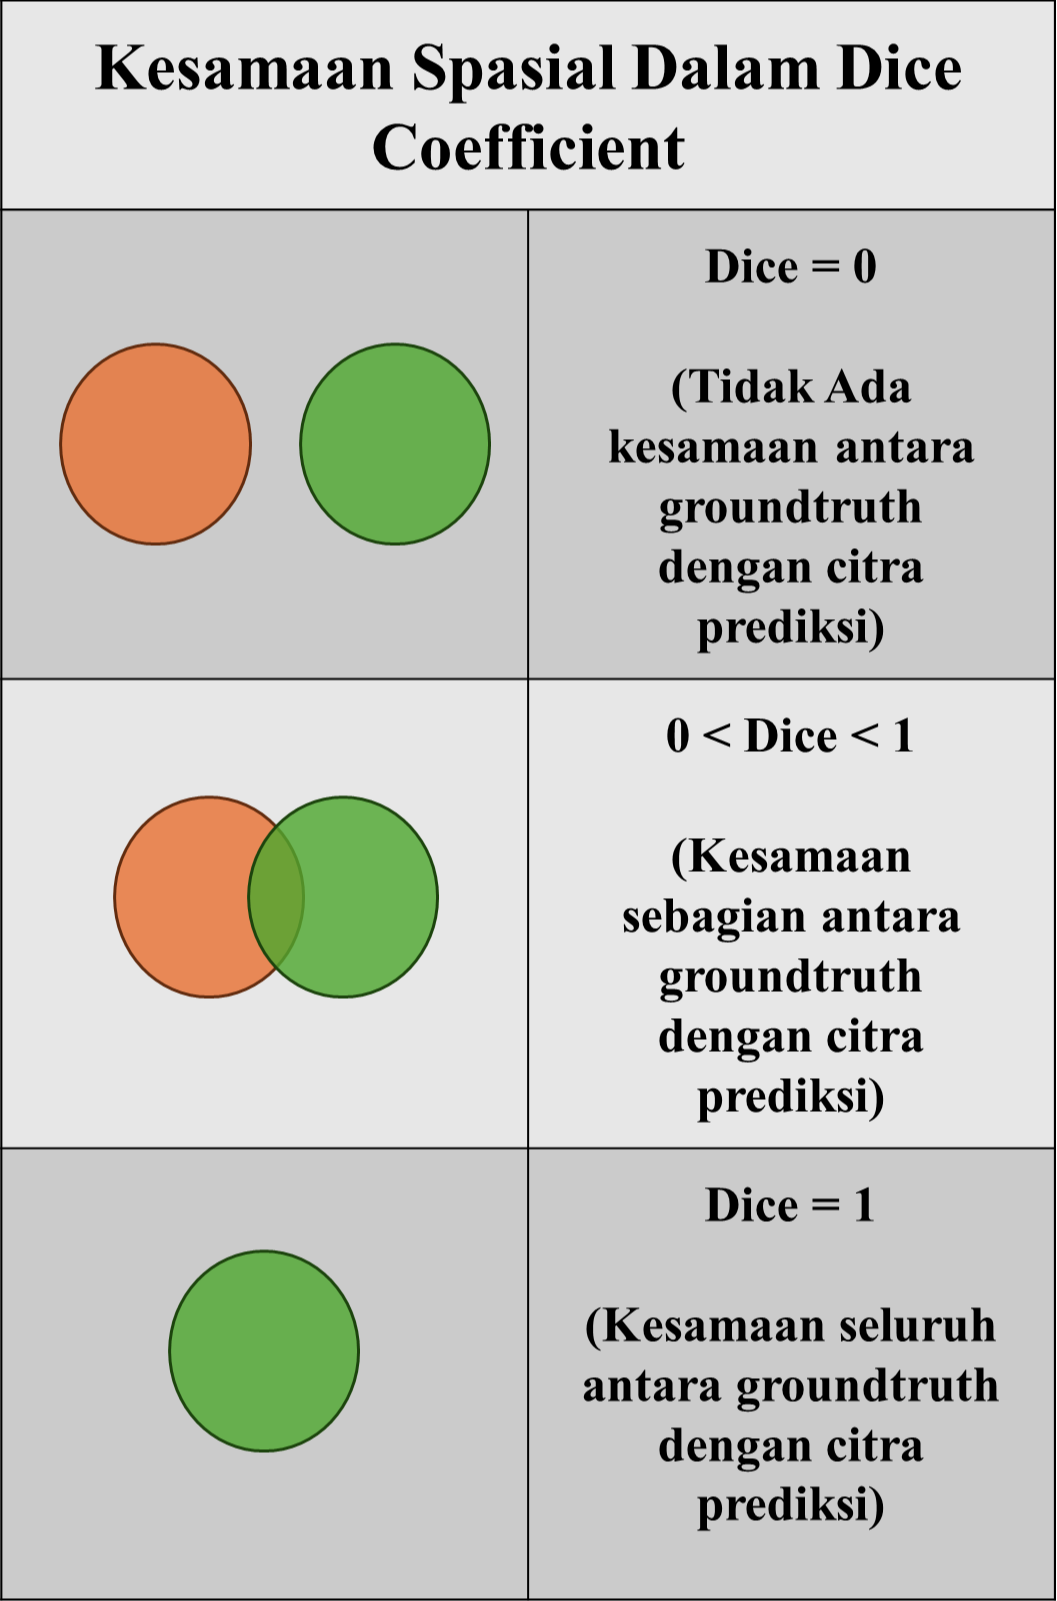
\includegraphics[scale= 0.2]{bab2/dice_spasial.png}
	\caption{Representasi Kesamaan dalam nilai \textit{dice coeffficient}}
	\label{fig:dice_spasial}
\end{figure}


\subsubsection{\textit{Hausdorff Distance}}
\textit{Hausdorff distance} merupakan metode pengukuran yang digunakan untuk menilai seberapa baik performa sebuah segmentasi citra, khususnya citra medis. Citra medis yang digunakan dalam peneltian ini adalah citra \textit{ultrasound}. Adapun cara kerja dari perhitungan \textit{hausdorff distance} yaitu menghitung jarak antara dua himpunan titik yang berasal dari 2 citra yaitu citra dengan area objek sebenarnya (\textit{groundtruth}) ($A$) dan citra dengan  area yang dihasilkan oleh model segmentasi (\textit{masking predicted})($B$). Adapun perhitungan \textit{hausdorff distance} dapat dirumuskan sebagai berikut. 

\begin{equation}
	hd(A,B)=max_{i,j}\left\{d(A_i,B), d(B_j, A)\right\}
	\label{eq13}
\end{equation}

Dimana,

\begin{equation}
	d(A_i,B)=min_{k}\left\{d(A_i,B_k)\right\}
\end{equation}

\begin{equation}
	d(B_j,A)=min_{k}\left\{d(B_j,A_k)\right\}
\end{equation} 

Berdasarkan definisi diatas, untuk menghitung jarak $d(A_i, B)$ menggunakan \textit{euclidean distance}. Variabel $hd(A, B)$ merupakan jarak terjauh yang ditempuh dari piksel $A$ ke bagian tepi dari $B$. Nilai \textit{hausdorff distance} yang rendah, yaitu mendekati 0, menunjukkan bahwa ada kemiripan yang tinggi antara objek - objek pada kedua citra tersebut. Hal ini dapat diartikan sebagai area prediksi dari hasil segmentasi sangat mirip dengan area sebenarnya (\textit{groundtruth}). Namun, apabila nilai \textit{haudorff distance} tidak mendekati 0, maka ada perbedaan yang signifikan antara dua titik. Sehingga terindikasi bahwa hasil segmentasi kurang akurat.



% \section{Cara Penulisan Persamaan}
% Cara menulis persamaan  inline pada text $\sum_{i=1}^{N} x_iy_i$


% Contoh Integral
% \begin{equation}\label{eq:persamaan1}
% y=\int_{0}^{2\pi} cos(x) dx
% \end{equation}
% Persamaan \ref{eq:persamaan1} adalah contoh menulis fungsi $cos(\alpha x)$ dari $0\le x\le 2\pi$.\\
% Menjajarkan persamaan
% \begin{align}
% y&=\int_{0}^{2\pi}cos(x)dx\\
% &=sin(x)|_0^{2\pi}\\
% &=sin(2\pi)-sin(0)\\
% &=0
% \end{align}
% Persamaan \ref{eq:matrix} adalah matrix.
% \begin{equation}\label{eq:matrix}
% \textbf{X}=\begin{bmatrix}
% x_{11}&x_{12}&\cdots&x_{1m}\\
% x_{21}&x_{22}&\cdots&x_{2m}\\
% \vdots&\vdots&\ddots&\vdots\\
% x_{n1}&x_{n2}&\cdots&x_{nm}
% \end{bmatrix}
% \end{equation}
% \vspace{1ex}
% \section{Cara Penulisan Tabel}
% \begin{table}[H]
% 	\caption{Tabel Contoh}
% 	\begin{tabular}{|l|l|l|l|}
% 		\hline
% 		No & X & Y & C \\ \hline
% 		1 & 0 & 0 & 1 \\ \hline
% 		2 & 0 & 1 & 0 \\ \hline
% 		3 & 1 & 0 & 0 \\ \hline
% 		4 & 1 & 1 & 0 \\ \hline
% 	\end{tabular}
% \end{table}


% \begin{table}[H]
% 	\label{tab:tabelcontoh2}
% 	\caption{Tabel ini contoh 2}
% 	\begin{tabular}{|l|l|l|l|}
% 		\hline
% 		\multirow{2}{*}{\textbf{No}} & \multicolumn{3}{l|}{\textbf{Data}} \\ \cline{2-4} 
% 		& \textbf{x} & \textbf{y} & \textbf{z} \\ \hline
% 		\textbf{1} & \textbf{0.1} & \textbf{0.2} & \textbf{0.3} \\ \hline
% 		\textbf{2} & \textbf{0.4} & \textbf{0.5} & \textbf{0.6} \\ \hline
% 	\end{tabular}
% \end{table}
% Pada Tabel \ref{tab:tabelcontoh2} di tunjukan cara membuat tabel.


% \begin{sidewaystable}
% 	\centering
% 	\caption{Tabel ke samping}
% 	\begin{tabular}{|l|l|l|l|}
% 		\hline
% 		\multirow{2}{*}{\textbf{No}} & \multicolumn{3}{l|}{\textbf{Data}} \\ \cline{2-4} 
% 		& \textbf{x} & \textbf{y} & \textbf{z} \\ \hline
% 		\textbf{1} & \textbf{0.1} & \textbf{0.2} & \textbf{0.3} \\ \hline
% 		\textbf{2} & \textbf{0.4} & \textbf{0.5} & \textbf{0.6} \\ \hline
% 	\end{tabular}
	
% \end{sidewaystable}
% \newpage
% \section{Cara Meletakan Gambar}
% \begin{figure}[H]
% 	\centering
% 	
\includegraphics[width=0.5\linewidth]{bab2/LambangTeknikElektro}
% 	\caption{Lambang Teknik dengan Ukuran 0.5 Lebar Kertas}
% 	\label{fig:lambangteknikelektro}
% \end{figure}
% \begin{figure}[H]
% 	\centering
% 	
\includegraphics[width=0.2\linewidth]{bab2/LambangTeknikElektro}
% 	\caption{Lambang Teknik dengan Ukuran 0.2 lebar kertas}
% 	\label{fig:lambangteknikelektro2}
% \end{figure}
% \begin{figure}[H]
% 	\centering
% 	
\includegraphics[width=0.5\linewidth]{bab2/LambangTeknikKOmputer}
% 	\caption{Lambang Teknik Komputer  }
% 	\label{fig:lambangteknikkomputer}
% \end{figure}
% \section{Cara Membuat  sitasi}

% Ini adalah cara  sitasi ke buku menggunakan cite\{Refferensi\}\\

% Contoh : sitasi ke 1
%  \cite{Brathwaite2009}.\\
% Daftar referensi terletak pada file 
% \textit{lainnya/pustaka.bib}\\

% contoh  sitasi ke 2
% \cite{Friedman1997}
% \newline
% \section{Algoritma}
% Contoh Algoritma

% \begin{algorithm}[H]
% 	\SetKwInOut{Input}{Input}
% 	\SetKwInOut{Output}{Output}
	
% 	\underline{function Euclid} $(a,b)$\;
% 	\Input{Two nonnegative integers $a$ and $b$}
% 	\Output{$\gcd(a,b)$}
% 	\eIf{$b=0$}
% 	{
% 		return $a$\;
% 	}
% 	{
% 		return Euclid$(b,a\mod b)$\;
% 	}
% 	\caption{Euclid's algorithm for finding the greatest common divisor of two nonnegative integers}
% \end{algorithm}
% \newpage
% \section{Tools Online Yang Cukup Membantu}
% Beberapa tools yang dapat digunakan untuk menulis tesis dengan latex.
% \subsection{Online equation editor: HostMath }
% \begin{center}
% 	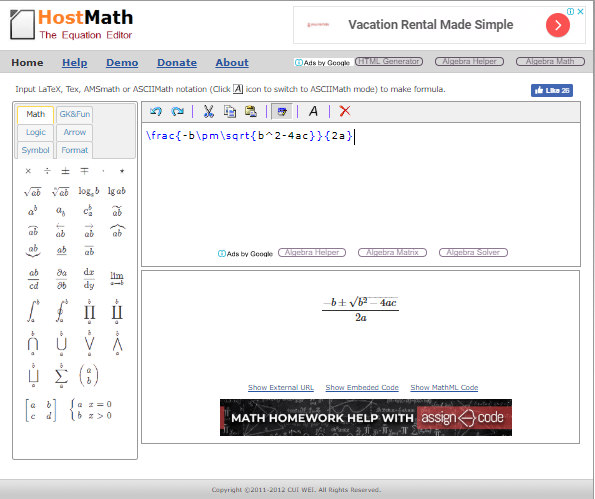
\includegraphics[width=1\linewidth]{bab2/Hosmath}
% 	\captionof{figure}{http://hostmath.com/}
% 	\label{fig:hosmath}
% \end{center}




% \newpage
% \subsection{Detexify LaTeX handwritten symbol recognition}
% \begin{center}
% 	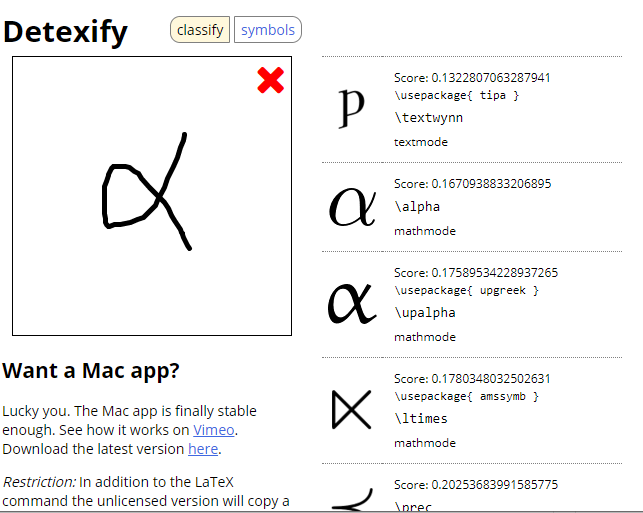
\includegraphics[width=\linewidth]{bab2/Detexify}
% 	\captionof{figure}{http://detexify.kirelabs.org/classify.html}
% 	\label{fig:detexify}
% \end{center}
% \newpage
% \subsection{Tables Generator }
% \begin{center}
	
% 	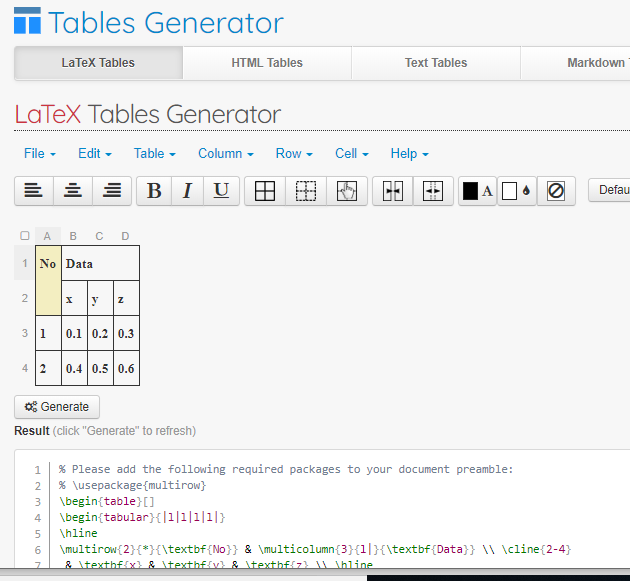
\includegraphics[width=0.7\linewidth]{bab2/TabelGenerator}
% 	\captionof{figure}{https://www.tablesgenerator.com/}
% 	\label{fig:tabelgenerator}
% \end{center}

% \subsection{Long Table}
% \begin{landscape}

% \begin{spacing}{1}	
% \begin{longtable}{|p{3cm}| p{7cm} | p{7cm} | p{7cm}|}\label{table:Posisidankontribusipenelitian}\\
% 	\caption{Posisi dan kontribusi penelitian}\\
% 	%\toprule
% 	\hline
% 	\nohyphens{\textbf{Topik riset Registrasi}}  & \textbf{Metode}  &\nohyphens{\textbf{Kontribusi Peneliti Lain}}&\nohyphens{\textbf{Kontribusi Peneliti}} \\ 
% 	%\midrule
% 	\hline
% 	\endfirsthead
% 	\caption{Posisi dan kontribusi penelitian \textit{(Lanjutan..)}}\\
% 	%\toprule
% 	\hline
	
% 	\nohyphens{\textbf{Topik riset Registrasi}}  & \textbf{Metode}  &\nohyphens{\textbf{Kontribusi Peneliti Lain}}&\nohyphens{\textbf{Kontribusi Peneliti}} \\ 
% 	%\midrule
% 	\hline
% 	\endhead
% 	\multicolumn{4}{r}{{(\textit{Tabel bersambung..})}} \\
% 	\endfoot
% 	\endlastfoot 
% 	Ekstraksi feature& 	Kurvature  pada suatu titik di hitung pada beberapa skala dengan fitting  permukaan ke  titik lokal pada berbagai macam ukuran. (Ho dan Gibbins, 2009) & 	Multi-scale  Feature Extraction from 3D Meshes and Unstructured Point Cloud& \\ \hline 
% 	Estimasi vektor normal& 	Fitting tangen vektor pada  data titik untuk menentukan vektor normal berbasis local voronoy mesh. (OuYang dan Feng, 2005) & 	Metoda baru untuk estimasi vektor normal. & \\ \hline 
% 	Estimasi principal direction& 	The Adjacent-Normal Cubic Approximation 
% 	(Goldfeather dan Interrante, 2004) & 	Estimasi principal direction dan vektor normal pada permukaan dengan noise yang tinggi.&\\ \hline 
% 	Registrasi berbasis fitur permukaan. & 	Normal distribution transform.
% 	(Pathak, Birk,Vaskevicius dan Poppinga, 2010) & 	Online registrasi pose untuk menentukan posisi robot. & 	 \\ \hline 
% 	Registrasi 3D berbasis warna. & 	Warna rgb (Johnson dan Kang, 1997). 
% 	(Douadi dkk., 2006) & 	Menggantikan fitur geometri ketika informasi geometri permukaan tidak mencukupi. & 	\\ \hline 
% 	& 	Registrasi berbasis warnoHSV. (Druon, Aldon dan Crosinier, 2006) & 	Registrasi tidak di pengaruhi oleh intensitas warna. & 	\\ \hline 
% 	& 	Registrasi dengan Modified color ICP kombinasi antara warna RGB dengan jarak ecludiean.  (Joun,Ang,Kang,Chung dan Yu(2009) & 	Registrasi untuk lingkungan 3D. & 	\\ \hline 
% 	Registrasi Berbasis geometri permukaan.& 	Registrasi dengan angular invariant feature.  (Jiang dkk., 2009) & 	\textit{Angular  invariant feature} invariant terhadap rotasi dan skala. & 	\\ \hline 
% 	& 	Point  Feature Histograms (PFH)  robust multi-dimensional features. (Rusu, Blodow, Marton, Soos dan Beetz, 2007) & 	Kombinasi curvature, vektor normal dan vektor pcincipal direction. & 	\\ \hline 
% 	& 	Fitting quadratik surface  (Chen dan Bhanu, 2007) & 	Permukaan lokal sebagai deskriptor untuk Kombinasi curvature, vektor normal dan vektor pcincipal direction. & 	\\ \hline 
% 	& 	& 	& 	Registrasi Citra  2D multiview untuk penangkap gerak manusia
% 	Semina Sesindo 2010 (Yuniarno, Mardi, Sumpeno dan Hariadi, 2010)\\ \hline 
% 	& 	& 	& 	Registrasi permukaan berbeasis surface curvature feature.
% 	Jurnal Jatit  (Yuniarno, Hariadi dan Purnomo, 2013a) \\ \hline 
% 	Outlier Removal& 	Tiga konstrain untuk memperoleh korspondensi akurat. 
% 	(Liu, 2008)& 	Korespondensi yang akurat& 	\\ \hline 
% 	& 	Dua  konstrain untuk memperoleh korspondensi akurat. 
% 	(Xin dan Pu, 2010)& 	Perbaikan tiga konstrain yang diusulkan oleh Liu dengan meletakan origin ke titik berat permukaan.& 	\\ \hline 
% 	& 	& 	& 	perbaikan korespondensi 
% 	dengan rigid constraint berbasis dua titik referensi dan surface curvature feature Jurnal Kursor (Yuniarno, Hariadi dan Purnomo, 2013b)\cite{Brathwaite2009} \\ \hline 
% \end{longtable}

% \end{spacing}

% \end{landscape}
% \section{Tabel Rencana Penelitian }


% \begin{table}[h!]
% 	\caption{Rencana Penelitian}
% 	\begin{tabular}{|l|l|l|l|l|l|l|l|l|l|}
% 		\hline
% 		& \multicolumn{9}{c|}{\textbf{Semester Ke}} \\ \cline{2-10} 
% 		\multirow{-2}{*}{} & 1 & 2 & 3 & 4 & 5 & 6 & 7 & 8 & 9 \\ \hline
% 		Rencana 1 & \cellcolor[HTML]{000000} & \cellcolor[HTML]{000000} & \cellcolor[HTML]{000000} & \cellcolor[HTML]{000000} & \cellcolor[HTML]{000000} &  &  &  &  \\ \hline
% 		Rencana 2 &  &  & \cellcolor[HTML]{000000} & \cellcolor[HTML]{000000} & \cellcolor[HTML]{000000} & \cellcolor[HTML]{000000} & \cellcolor[HTML]{000000} &  &  \\ \hline
% 		Rencana 3 &  &  &  &  &  & \cellcolor[HTML]{000000} & \cellcolor[HTML]{000000} & \cellcolor[HTML]{000000} & \cellcolor[HTML]{000000} \\ \hline
% 		Rencana 4 &  & \cellcolor[HTML]{000000} & \cellcolor[HTML]{000000}{\color[HTML]{000000} } & \cellcolor[HTML]{000000}{\color[HTML]{000000} } & \cellcolor[HTML]{000000}{\color[HTML]{000000} } & \cellcolor[HTML]{000000}{\color[HTML]{000000} } & \cellcolor[HTML]{000000}{\color[HTML]{000000} } & \cellcolor[HTML]{000000}{\color[HTML]{000000} } & \cellcolor[HTML]{000000}{\color[HTML]{000000} } \\ \hline
% 	\end{tabular}
% \end{table}



